\documentclass{article}
\usepackage[utf8]{inputenc}
\usepackage{graphicx}
	\DeclareGraphicsExtensions{.png, .jpeg}
\usepackage[top=1in, bottom=1in, left=1in, right=1in]{geometry}

\title{Compiler Construction \\ WA01: Regular Expressions and FSMs}
\author{Terence Henriod}
\date{\today}

\begin{document}

\clearpage            % All of
\maketitle            % this,
\thispagestyle{empty} % removes the page number from the title page

\begin{abstract}
\noindent This assignment asks you to prepare written answers to questions on regular languages
and finite automata. Each question has a short answer. You may discuss this assignment
with other students and work the problems together. However, your writeup should be your
own individual work. Remember written assignments are to be turned in in class on the date
due.
\end{abstract}

\newpage

\begin{enumerate}
  \item Write regular expressions for the following languages:
  \begin{enumerate}
    \item (2 points) All strings of $a$s and $b$s that do not include the
          substring $ab$.\\\\
      \textit{Answer}:\\\\
      $b^{*}a^{*}$\\

    \item (2 points) All strings of $a$s and $b$s that do not include the
          substring $aba$.\\\\
      \textit{Answer}:\\\\
      $(b^{*}(a^{*}b^{*} | a^{+}bb^{+}))^{*}$\\

    \item (2 points) All strings of digits where every 3rd digit (starting
          with the first digit) is even.\\\\
      \textit{Answer}: \\\\
      Assumption: the pattern of digits will look like
      $any, even, even, any, even, even, ...$.\\
      Assumption: for the string to be a ``string of digits," it must be non-empty.\\\\
      Let $e = (0|1|2|3|4|5|6|7|8|9)$, and $a = (0|2|4|6|8)$, then the solution is\\
      $(eaa)^{+} | ea | e$\\
  \end{enumerate}

  \item For each of the following finite automata, give an equivalent regular
        expression.\\\\
  \begin{enumerate}
    \item (2 points)
    \begin{figure}[h]
	\centering
	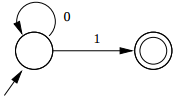
\includegraphics[width=0.25\textwidth]{WA01_2a}
        % extension usually unnecessary when specifying file
	% \caption{A bad robot.}
	\label{fig:WA01_2a}
	\end{figure}
    \\\\
      \textit{Answer}:\\\\
      $0^{*}1$\\

    \item (2 points)
    \begin{figure}[h]
	\centering
	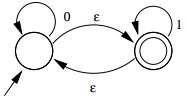
\includegraphics[width=0.25\textwidth]{WA01_2b}
        % extension usually unnecessary when specifying file
	% \caption{A bad robot.}
	\label{fig:WA01_2b}
	\end{figure}\\\\
      \textit{Answer}:\\\\
      $(0^{*}1^{*})^{*}$\\

    \newpage
    \item (2 points)
    \begin{figure}[h]
	\centering
	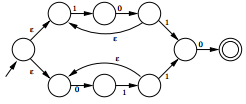
\includegraphics[width=0.4\textwidth]{WA01_2c}
        % extension usually unnecessary when specifying file
	% \caption{A bad robot.}
	\label{fig:WA01_2c}
	\end{figure}\\\\
      \textit{Answer}:\\\\
      $((10)^{+} | (01)^{+})10$\\

  \end{enumerate}

  \item (3 points) Let $\Sigma = a, b$. How many DFAs are there with two states and input alphabet $\Sigma$? (Note: Many of these machines may accept the same language. Count DFAs as different if the machines are different, even if they accept the same language.)\\\\
  \textit{Answer}:\\\\
  This is essentially a combinatorial problem. In order to proceed, it would be good to state some facts and clarify some assumptions. First, we should state that since this is a DFA, there will be no arcs associated with any $\epsilon$ transitions, obviously. Also, every symbol in an alphabet must be associated with one, and only one, outgoing edge at from vertex (state of the machine), whether the edge is a self-edge or otherwise. The assumption that the machine does not need to be ``functional" or ``optimal" is made, meaning that the machine does not necessarily have to accept any language or that all states are reachable. The final assumption, although not necessary to our analysis, is that states of the machine may be of only two types: accepting or non-accepting.

  Now, onto solving the problem. Let's start by numbering the types of machines we can have based on which states are accepting and non-accepting. If there are $n$ states in the machine, each state can be any of $m$ types. Thus there will be $m^n$ types of machines based on state types.

  Next, we need to determine the number of ways that the transitions from each state can be arranged. Each letter of the accepted alphabet could be assigned to an edge representing a transition to any of the $n$ states (including the self-edge representing staying). Thus if the alphabet is of size $p$, there are $p * n$ ways to transition for each state. Since there are $n$ states, there must be $n^{pn}$ ways to to organize all of the transitions. (Imagine that each state is a digit in a number and each digit could take a different value for each way to transition from the state.)

  Finally, the starting state of the machine can be any of the $n$ nodes.

  Finally, putting it all together, if we consider all of the ways to start in the maching, for each way to type the states, for each way to organize the transitions, then we have the number of possible DFAs is $n * m^{n} * n^{pn}$.

  In the case of our problem, we have $n = 2$ states, an alphabet size $p = 2$, and a number of state types $m = 2$. Plugging and chugging gives:
  $$n *m^{n} * n^{pn} = (2) * (2)^{(2)(2)} * (2)^{(2)} = 2 * 2^{4} * 2^{2} = 2 * 16 * 4 = 128$$
\end{enumerate}

\end{document}
